\section{Background}

\begin{frame}{Regularization Alleviates Overfitting}

\begin{figure}
\subcaptionbox{without regularization}[.48\textwidth]{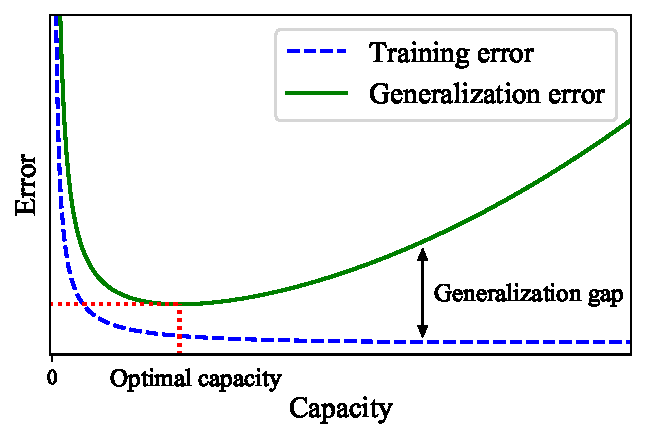
\includegraphics[width=.48\textwidth]{figs/gap1.pdf}}
\subcaptionbox{with regularization}[.48\textwidth]{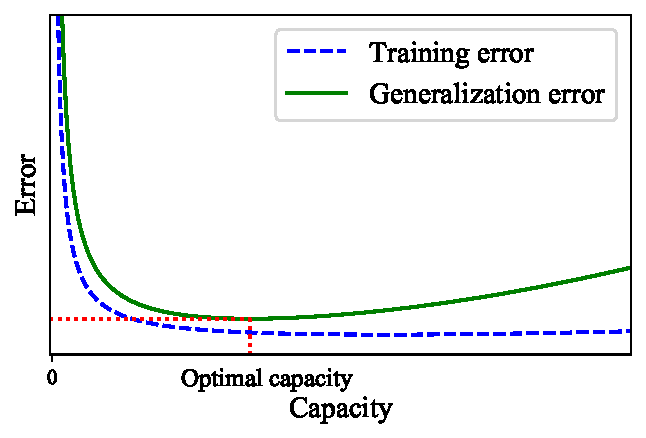
\includegraphics[width=.48\textwidth]{figs/gap2.pdf}}
\end{figure}

\end{frame}

\begin{frame}{Flat Minima Helps Generalization}

\begin{itemize}
    \item Flat minima correspond to low-complexity networks. (Hochreiter \etal, 1997)
    \item Small-batch SGD produces flat minima that generalize well. (Keskar \etal, 2017)
    \item Better minimizers of loss function are flatter in visualization. (Li \etal, 2018)
    \item A PAC-Bayes based generalization guarantee for flat minima. (Foret \etal, 2020)
\end{itemize}

\begin{figure}
\subcaptionbox{ResNet without skip connections}[.48\textwidth]{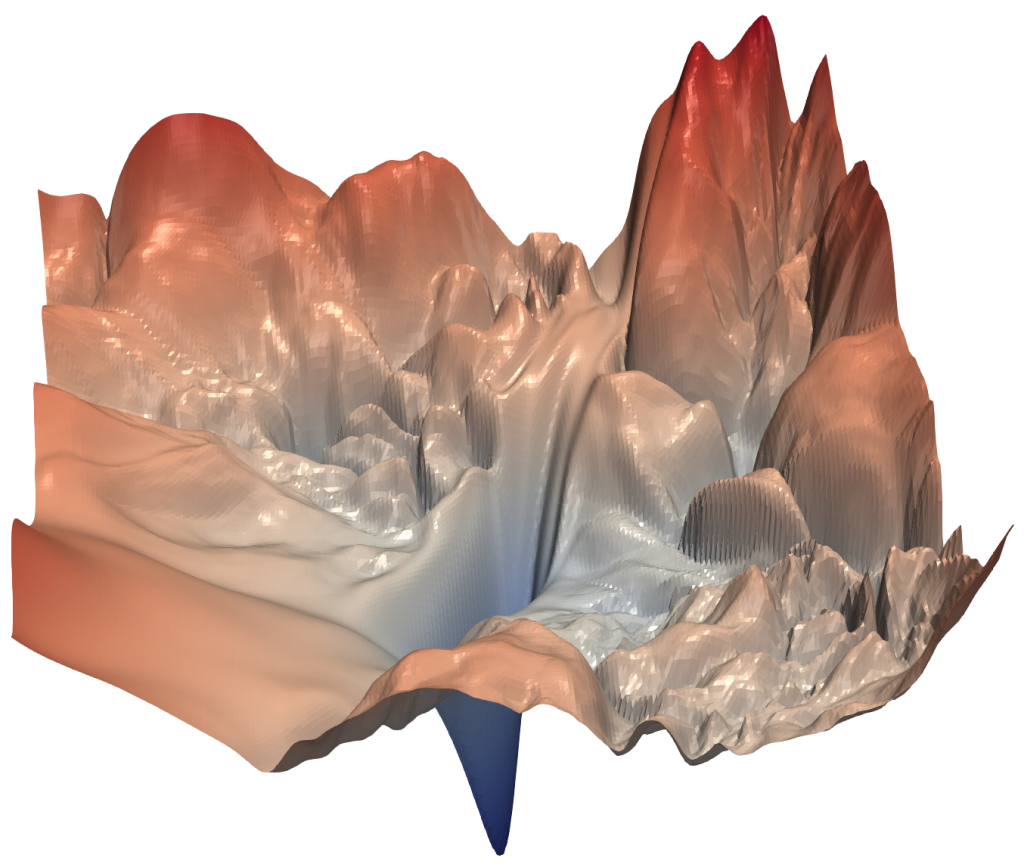
\includegraphics[width=.25\textwidth]{figs/flatness_a.png}}
\subcaptionbox{ResNet with skip connections (Li \etal, 2018)}[.48\textwidth]{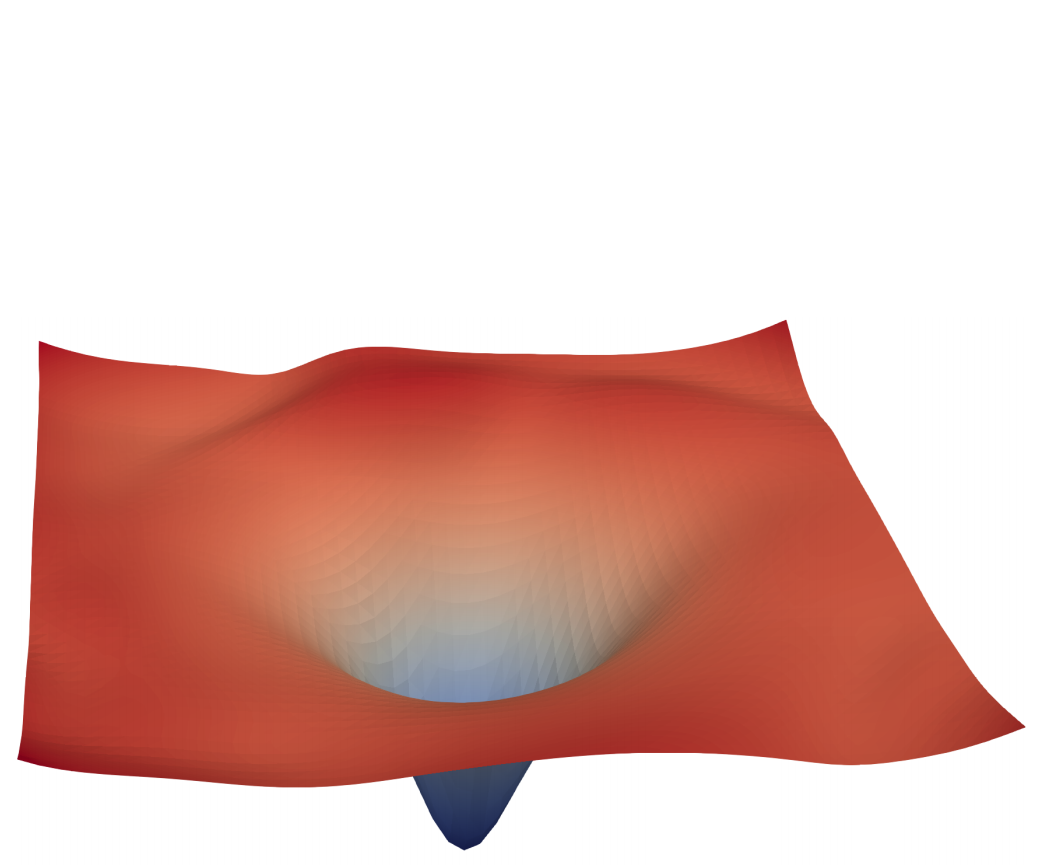
\includegraphics[width=.25\textwidth]{figs/flatness_b.png}}
\end{figure}
\end{frame}
